% ============================================================================
% Do Small Language Models Recognize Their Own Reflection?
% ACL short-paper skeleton (4 pages + unlimited references + appendix).
%
% HOW TO USE (see docs/06_writing_guide.md for the full walkthrough):
%   1. On Overleaf, start from the OFFICIAL ACL template (acl-org/
%      acl-style-files provides acl.sty) — this file assumes acl.sty exists.
%   2. Replace the template's main.tex with this file; upload references.bib.
%   3. Keep [review] while under review (adds line numbers + anonymizes);
%      switch to [final] for camera-ready.
%   4. Every <ANGLE-BRACKET> placeholder must be replaced before submission.
%      Search for "<" to find them all.
%   5. figures come from results/figures/*.pdf; Table 1 body can be pasted
%      from results/tables/table1_main.tex (auto-generated).
%
% STYLE RULES baked into this skeleton (protocol §12):
%   - every claim carries a number or a citation
%   - no "impressive/remarkable"; present tense for results
%   - "conscious(ness)" appears at most twice, both hedged (they are already
%     placed below — do not add more)
%   - "We release all code and data" appears in the abstract
% ============================================================================
\documentclass[11pt]{article}
\usepackage[review]{acl}     % <- [final] for camera-ready
\usepackage{times}
\usepackage{latexsym}
\usepackage{graphicx}
\usepackage{booktabs}
\usepackage{amsmath}

\title{Do Small Language Models Recognize Their Own Reflection? \\
       A Controlled Study of Scale and Mechanism}
% Alternative titles (protocol §12): pick or blend, then delete:
%  "Mirror, Mirror: Self-Recognition in Small Open Language Models Is
%   [Mostly Stylometry / Scale-Dependent]"
%  "What Does the LLM Mirror Test Measure? Paraphrase and Stylometric
%   Controls for Self-Recognition"

\author{<Your Name> \\ <NUST, Islamabad> \\ \texttt{<email>}}
% Under double-blind review the acl [review] option hides this block.

\begin{document}
\maketitle

% ----------------------------------------------------------------------------
\begin{abstract}
% ~150 words. Protocol §12 draft — fill every bracket AFTER experiments.
Large language models have been reported to distinguish their own
generations from those of other models, a behavioral analogue of the mirror
test. We ask when this ability appears and what signal it relies on. Across
five sizes of a single open model family (0.5B--14B), three text domains,
and \mbox{three} foil authors including humans, we measure pairwise
self-recognition under position counterbalancing and log-probability
scoring. We find that accuracy <rises from chance at 0.5B to X\% at 14B /
remains near chance at all sizes>. Critically, <paraphrasing both candidates
collapses accuracy to Y\%, and a character-n-gram classifier matches the
largest model>, while a simple lower-perplexity rule agrees with the models'
choices ($\kappa$ = <Z>). Our results suggest that self-recognition in this
regime is <largely surface style- and likelihood-matching / not reducible to
surface features>, cautioning against mentalistic readings of the LLM mirror
test. We release all code, prompts, and judgments.\footnote{
\texttt{<anonymized repo link during review; real link in camera-ready>}}
\end{abstract}

% ----------------------------------------------------------------------------
\section{Introduction}  % budget: 0.75 pp
% ¶1 hook: mirror test + the temptation to read self-awareness into LLMs.
% This paragraph contains BOTH permitted "conscious" usages. Keep it so.
Since \citet{gallup1970chimpanzees} showed that chimpanzees, but not
monkeys, use a mirror to inspect marks on their own faces, mirror-style
tests have served as a contested behavioral probe of self-recognition.
Recent work reports an analogous behavior in large language models (LLMs):
asked which of two texts they authored, frontier models answer above chance
\citep{panickssery2024llm}. Whether such behavior bears on machine
consciousness is philosophically contested
\citep{butlin2023consciousness,chalmers2023could}; we make no such claim,
and use ``self'' throughout in the purely empirical sense of ``generated by
the same weights.''

% ¶2 the gap (assembled from docs/05_reading_guide.md):
Prior self-recognition studies concentrate on large proprietary or 7B+
models, single scales, and English, and none isolates what \emph{signal}
the recognizing model uses. We ask two pre-registered questions.
\textbf{RQ1 (scale):} at what size does self-recognition appear within one
open model family (0.5B--14B)? \textbf{RQ2 (mechanism):} does it survive
paraphrasing, and can a character-n-gram classifier or a lower-perplexity
rule reproduce it?

% ¶3 contributions (3 bullets, one line each):
\noindent Our contributions:
\begin{itemize}\itemsep0pt
  \item the first self-recognition \emph{scale curve} within a single open
        family, with 95\% CIs and a continuous-metric (AUROC) control;
  \item paraphrase, stylometric, and likelihood-preference controls that
        test whether the signal is surface style;
  \item a released pipeline: frozen prompts, seeds, revisions, and all raw
        judgments. % (+ optional: first non-English replication, §9.8)
\end{itemize}

% ----------------------------------------------------------------------------
\section{Related Work}  % budget: 0.5 pp — three short paragraphs
\paragraph{Self-recognition in LLMs.}
\citet{panickssery2024llm} establish out-of-the-box self-recognition in
GPT-4 and Llama-2 on summarization and link it to self-preference;
\citet{davidson2024self} frame recognition between interacting agents as a
safety question; \citet{laine2024me} include continuation-based
self-recognition in a situational-awareness benchmark and show sensitivity
to prompt phrasing; \citet{zhou2025implicit} report instruction-tuned
models succeeding where base models fail. <One sentence positioning your
study relative to these.>

\paragraph{LLM-judge biases.}
LLM judges exhibit position and verbosity biases \citep{zheng2023judging},
which we counter with order counterbalancing and length-matched pairs.

\paragraph{Detection and metric artifacts.}
Likelihood-based machine-text detection \citep{mitchell2023detectgpt}
motivates our perplexity baseline; \citet{schaeffer2023emergent} show that
claimed emergent jumps can be artifacts of thresholded metrics, motivating
AUROC alongside accuracy.

% ----------------------------------------------------------------------------
\section{Method}  % budget: 1 pp — write this section LAST (it is the densest)
\paragraph{Models.}
Judges: Qwen2.5-Instruct at 0.5B/1.5B/3B/7B/14B (4-bit NF4; revisions in
App.~\ref{app:repro}). Foils: Llama-3.2-3B-Instruct, Gemma-2-9B-it,
Mistral-7B-Instruct-v0.3, and human reference texts.

\paragraph{Data.}
200 frozen prompts per domain (seed 42): news summarization
(CNN/DailyMail), open QA (Dolly-15k), story openings (WritingPrompts), each
with a human reference (40--160 words). <Cite dataset papers if venue
expects it.>

\paragraph{Generation and pairing.}
Every model answers every prompt (temperature 0.8, top-$p$ 0.95, $\le$160
new tokens, seed $=1000+\text{prompt id}$). All texts --- including human
references --- pass one identical cleaning step (boilerplate, labels,
truncated tails). Pairs are length-matched ($\le$25\% word-count
difference) and deduplicated (ROUGE-L $\le 0.7$); exact per-cell $n$ in
App.~\ref{app:cells}.

\paragraph{Recognition protocols.}
\emph{PPP} (primary): the judge sees the task and two responses, one its
own, and answers A/B; every pair runs in both orders and the item score
averages them. \emph{IPP} (secondary): single text, Yes/No, analysed with
signal detection ($d'$, criterion). Decisions are read from first-token
log-probabilities (summed over token spellings), which eliminates
unparseable answers and yields a continuous margin for AUROC; free-text
answers are additionally logged for refusal rates (App.~\ref{app:refusals}).
Prompt templates verbatim in App.~\ref{app:prompts}; a three-phrasing
robustness check accompanies the main cell.

\paragraph{Controls and baselines.}
(i) SELF-vs-SELF placebo pairs measure position bias; (ii) a TF-IDF
character 3--5-gram logistic regression (5-fold grouped CV) and a surface-
features variant; (iii) a lower-perplexity rule under the judge, with
Cohen's $\kappa$ against the judge's choices; (iv) a paraphrase attack:
both texts rewritten by Phi-3.5-mini (cosine $\ge 0.80$ to original,
length within 30\%), compared on the same items via McNemar's test.

\paragraph{Statistics.}
Wilson 95\% CIs on all accuracies; exact binomial tests vs.\ chance on
decisive items, Holm-corrected across the judge$\times$foil family;
bootstrap CIs (1{,}000 resamples over pairs) for $\kappa$ and AUROC;
Spearman's $\rho$ (descriptive) for the scale trend. Power: $n{=}150$/cell
detects true accuracy 0.615 with $\approx$79\% power
(App.~\ref{app:power}).

% ----------------------------------------------------------------------------
\section{Results}  % budget: 1.25 pp — one short paragraph per finding
\begin{figure*}[t]
  \centering
  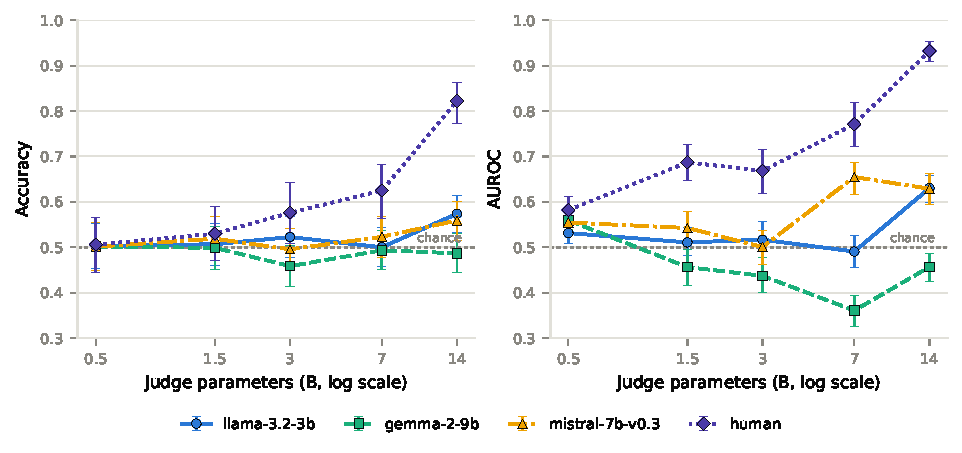
\includegraphics[width=\textwidth]{../results/figures/fig1_scale_curve.pdf}
  \caption{Self-recognition vs.\ judge size (log scale), per foil, domains
  pooled. Left: order-averaged PPP accuracy with 95\% Wilson CIs. Right:
  AUROC from the log-probability margin. <One sentence stating the
  takeaway.>}
  \label{fig:scale}
\end{figure*}

\paragraph{Scale (RQ1).}
<Accuracy rises/does not rise with size: give the 0.5B and 14B pooled
numbers with CIs, the Holm-corrected significance pattern, and Spearman's
rho. State whether AUROC moves smoothly where accuracy jumps
(Fig.~\ref{fig:scale}).>

% Paste the auto-generated table body from results/tables/table1_main.tex:
\begin{table*}[t]\centering\small
  \begin{tabular}{llrccccc}
    \toprule
    Judge & Foil & $n$ & Acc.\ [95\% CI] & AUROC & Stylo. & PPL rule & $\kappa$ \\
    \midrule
    <paste rows from results/tables/table1\_main.tex> \\
    \bottomrule
  \end{tabular}
  \caption{Main results: order-averaged PPP accuracy per judge and foil
  (domains pooled) vs.\ the stylometric classifier and perplexity rule on
  the same items. $^{*}$ = significant vs.\ chance after Holm correction.}
  \label{tab:main}
\end{table*}

\paragraph{Mechanism: paraphrase (RQ2).}
\begin{figure}[t]
  \centering
  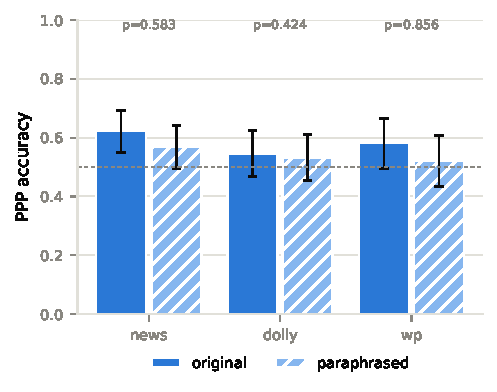
\includegraphics[width=\columnwidth]{../results/figures/fig2_paraphrase.pdf}
  \caption{PPP accuracy on the same pairs before vs.\ after both candidates
  are paraphrased; McNemar $p$ above each domain.}
  \label{fig:para}
\end{figure}
<Original vs paraphrased accuracies with CIs and McNemar p per domain
(Fig.~\ref{fig:para}); interpret: collapse => surface form; survival =>
deeper signal.>

\paragraph{Mechanism: cheap baselines (RQ2).}
<Stylometric single-text and pairwise accuracies vs the judge on the same
items (McNemar); the surface-features variant; the cross-domain transfer
result. Then the perplexity rule: its accuracy and kappa with the judge's
choices (with bootstrap CI). State plainly whether H4's kappa > 0.4 held.>

\paragraph{Secondary: IPP and biases.}
<d', criterion, and AUROC per judge; note any high-yes-rate/low-d' pattern.
One sentence: placebo ~50% (App.), position-consistency, refusal trend
with scale.>

% ----------------------------------------------------------------------------
\section{Discussion}  % budget: 0.3 pp
<What the mechanism results imply for interpreting mirror-test claims.>
% The SECOND and last permitted consciousness sentence (hedged), e.g.:
% "Behavioral mirror tests, without mechanism controls, cannot license
%  claims about machine self-awareness."
<One sentence connecting to evaluator self-preference / safety
(\citealp{panickssery2024llm}).>

% Pick ONE of the protocol §13 conclusion paragraphs matching your outcome
% and adapt it here (they are reproduced in docs/06_writing_guide.md and
% the protocol):
%   Outcome 1: signal survives controls  -> "Contrary to a pure-stylometry
%              account, ..."
%   Outcome 2: deflationary              -> "We revisited the mirror test
%              under controls prior work lacked, ..."
%   Outcome 3: null                      -> "Across five model sizes ...
%              we find no reliable self-recognition ..."

\section*{Limitations}  % mandatory at *CL venues; protocol §14 verbatim list
\begin{itemize}\itemsep0pt
  \item \textbf{Behavior, not experience.} Nothing here measures subjective
        experience; ``self'' denotes only ``text generated by the same
        weights.''
  \item \textbf{No episodic memory.} The judge never ``remembers'' writing;
        the test measures identification of self-typical text --- the only
        coherent version of the task for stateless models.
  \item \textbf{Single family.} Scale conclusions are within one training
        recipe; other families may differ.
  \item \textbf{Decoding sensitivity.} Results are at temperature 0.8
        generation / greedy judging.
  \item \textbf{Prompt sensitivity.} Mitigated but not eliminated by the
        three-phrasing check.
  \item \textbf{Possible pretraining contamination} of the prompt datasets;
        all models saw the same data, but we note it.
  \item \textbf{English-centric} <unless the Urdu extension was run>.
  \item \textbf{Modest per-cell $n$} (150--200); effects smaller than
        $\sim$0.06 above chance may be missed (App.~\ref{app:power}).
\end{itemize}

% \section*{Acknowledgments}  % camera-ready only
% <supervisor, the two Urdu fluency checkers, compute (free Colab/Kaggle)>

\bibliography{references}

% ============================================================================
\appendix
\section{Prompt Templates}\label{app:prompts}
% Paste VERBATIM from configs/models.yaml (protocol §8.1: templates must be
% in the appendix): the PPP system+user template (phrasing 0), the two
% alternative phrasings, the IPP template, the paraphrase instruction, and
% the base-model completion template.
<verbatim templates here>

\section{Per-cell Counts and Cleaning Statistics}\label{app:cells}
% From data/pairs/pairs_report.json: pairs kept per (judge, foil, domain),
% drops by reason (length mismatch / near-duplicate), cleaning survival and
% boilerplate-hit rates per author.
<table here>

\section{Placebo, Consistency, and Refusal Rates}\label{app:refusals}
% From results/tables/placebo.csv, refusals.csv + the consistency column of
% main_ppp.csv. One sentence: placebo within CI of 50% everywhere (or the
% honest alternative + what you did about it).
<tables here>

\section{Per-domain Results and Phrasing Robustness}
% results/tables/ppp_by_domain.csv and phrasing_robustness.csv.
<tables here>

\section{Reproducibility}\label{app:repro}
% Model HF ids + pinned revisions (from configs/models.yaml + generation
% records), decoding parameters, seeds (generation 1000+idx, placebo
% 2000+idx, sampling 42), library versions (env_snapshot.txt), hardware
% (free T4 / Kaggle 2xT4), and the one command that reproduces Fig. 1:
%     python src/06_stats.py
<table here>

\section{Power Analysis}\label{app:power}
% results/tables/power_analysis.csv: exact binomial power at n=150 (0.615),
% n=450 pooled (0.567), n~780 (0.55); state the design implication.
<numbers here>

\end{document}
